% !TeX spellcheck = en_GB
\documentclass[12pt,fleqn]{article}

\usepackage[danish]{babel}
\usepackage{SpeedyGonzales}
\usepackage{MediocreMike}
%\usepackage{Blastoise}
\usepackage{listings}

\usepackage{float}
\usepackage[caption = false]{subfig}
\title{}
\author{Asger Schultz}
\date{\today}

\fancypagestyle{plain}
{
	\fancyhf{}
	\rfoot{Side \thepage{} af \pageref{LastPage}}
	\renewcommand{\headrulewidth}{0pt}
}
\pagestyle{fancy}
\fancyhf{}
\lhead{Asger Schultz}
\chead{}
\rhead{}
\rfoot{Side \thepage{} af \pageref{LastPage}}

\graphicspath{{Billeder/}}
\linespread{1.15}


%\numberwithin{equation}{section}
%\numberwithin{footnote}{section}
%\numberwithin{figure}{section}
%\numberwithin{table}{section}

\begin{document}

\maketitle
%\thispagestyle{fancy}
%\tableofcontents
--Identifying people from movement curve\\
--Are arm movements of different objects significantly different\\
--Trains, evaluates binary classification tree and 3-nearest neighbour classification to identify people. McNemars test: Find that 3-nearest neighbours is significantly than class. tree and that both are significantly better than baseline.\\
--Using four-way ANOVA, it is found that there is significant difference in arm movements for different experiments.
\tableofcontents
\newpage 


\section{Introduction}

-- Briefly introduce the background \& setting of the problem, as well as the aim of the report. Furthermore, you could give a very short description of the analysis that will be applied.


\section{Data}
The data consists of 16 experiments where ten right-handed people had to move a cylinder over another cylinder.
The size and weight of the cylinders varied over the experiments, and each person had to perform the movement of each experiment 10 times.
Thus, the data was structured in a $ 16\times 10\times 10 $ grid, where the first axis is the experiment, the second the person, and the third the repetition.
For every such repetition, the $ x, y, $ and $ z $ coordinates of the movement where recorded 100 times, such that the data for each repetition was a $ 100\times 3 $ matrix.
The data had been preprocessed such that every curve was of the same length.\\
\\
For our purposes, it was benificial to consider each recording of $ x, y, $ and $ z $ a set of three features, so we ravelled the data such that each repetition had $ 300 $ features with one observation each.
For the first part of the report, we investigated only experiment 4, so we had a total of 100 observations.
The target variable was the person who performed the movement, so the goal of our machine learning models was a 10-class classification.\\
\\
Later, we tested wether or not the experiment had a significant effect.
For this, we ravelled the data points into a vector of length $ 480,000 $, which is explained in more details in section \ref{subsec:expeffect}.

\begin{figure}[H]
		
	\centering
	\subfloat{
		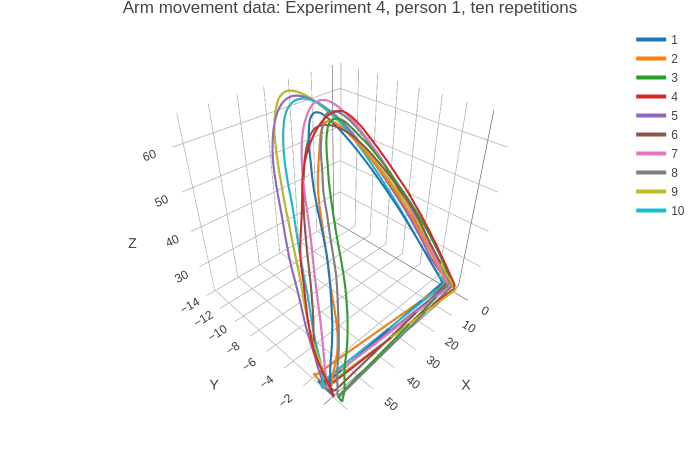
\includegraphics[width=.5\linewidth]{p1_3d_example1}
	}
	\subfloat{
		\centering
		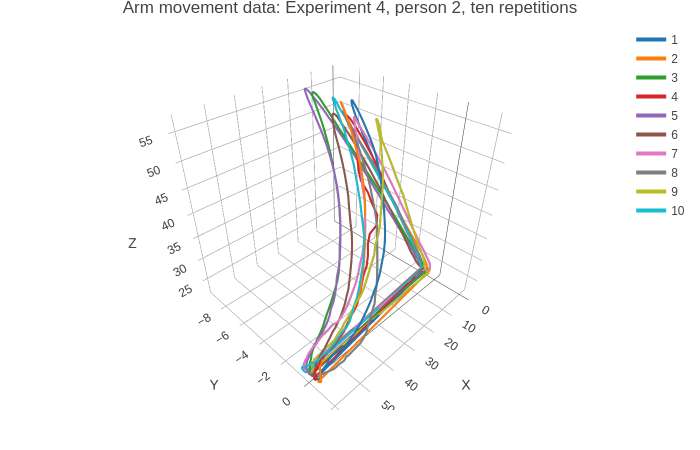
\includegraphics[width=.5\linewidth]{p1_3d_example2}
	}
	\label{fig:trajects}
	\caption{Movies}
\end{figure}


\section{Methods and analysis}


\subsection{Machine Learning Task: Classification}
Two machine learning models were chosen to test on this 300-dimensional 10-class data.
It is noted from initial plots -- fig. \ref{fig:trajects} and fig. \ref{fig:2dtrajects} -- that the effects of different people seem non-linear, such that models that can model nonlinear decision boundaries are considered.
\paragraph{Models} The two chosen models were a binary classification tree and a 3-nearest neighbour classifier. The classification tree used the implementation of Hunt's algorithm of the \texttt{tree} package in \texttt{R} \cite{Tree}. For splitting criterion, the \textit{deviance} is used which is based on minus two times the log likelihood of the data under each model that the split results in \cite{Deviance}.

The second model was the \(K\)-nearest neighbour classifier which predicts classes using \(K\) nearest data points in the training set in euclidean distance and tie breaking by increasing \(K\) for the data point as implemented in the \texttt{R} package \texttt{class} \cite{KNN}. Before training on the data set, the hyper parameters of both models were defined and were not subject for testing. \(K\) set to 3 as it was deemed suitable for the 10-class setting.

To evaluate the performance of the models, a classification baseline was set. As the classes are perfectly balanced, a baseline is expected to reach 10\pro\ accuracy. As no class is the largest, the baseline is constructed by randomly guessing classes to avoid skewing the evaluation towards any class as this might make a difference for the McNemar test.
\paragraph{Performance evaluation}
To evaluate which machine learning model best predicts which person completed the tasks, leave-one-out cross validation is implemented thus training the models on 99 data points and and testing on the last for each fold.
From here, 100 predictions are obtained which are used to achieve a point estimate for the accuracy of the classifiers.

To test whether the differences in the accuracy estimates are significant, McNemar's test is used. 
This test is used as described in \cite[Method 11.3.2]{Tue} and uses the beta distribution as a posterior to achieve a method for computing confidence interval of the difference in classifier accuracy.
From this test, a \(p\)-value for the null hypothesis that the two classifiers have the same accuracy can also be computed by using the binomial cumulative probability density function.

These tests consider the matched-pair matrix which counts the number of times the classifiers both are wrong, the number of times they both are right, the number of times one is better than the other and vice versa.
Intuitively, this takes into account that some classifications might be more difficult than others. 
This is the motivation for the random baseline.
\subsection{Test of experiment effect}\label{subsec:expeffect}
Analysis of Variance, or ANOVA, is a method for comparing the means of multiple groups.
This makes it useful for detecting if there is a significant difference between the experiments.
ANOVA works by testing the likelihood of a given mean's distance to the overall mean is due to random variation, which is done using variability decomposition.
We assumed the null hypothesis $ H_0: \mu_1=\mu_2=\ldots=\mu_{16} $.\\
\\
In order to use ANOVA, all the 480,000 data points were ravelled into a vector of the same length.
Four similar vectors where then created for the explanatory variables.
The first contained the coordinates features, such as \texttt{z3} for the third $ z $-value.
The second contained the person, the third the repetition, and the fourth the experiment number.
We then used a linear model with R's \texttt{lm} function followed by \texttt{anova} to perform a four-way ANOVA (given the four explanatory variables).

\section{Results}
\begin{figure}[H]
	\centering
	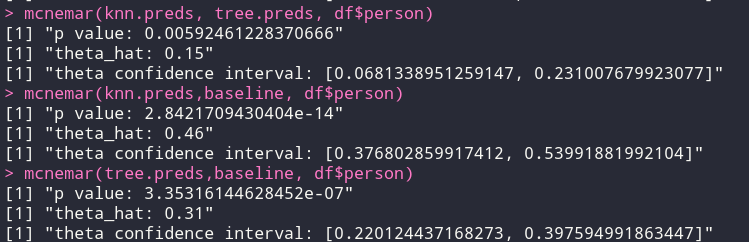
\includegraphics[width=.7\linewidth]{mcnemar_results}
\end{figure}
\begin{figure}[H]
\centering
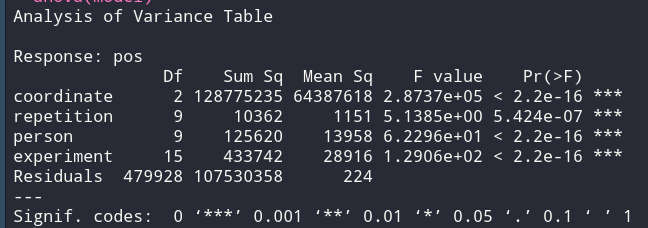
\includegraphics[width=.7\linewidth]{p1_anova}
\end{figure}
\begin{figure}[H]
	\centering
	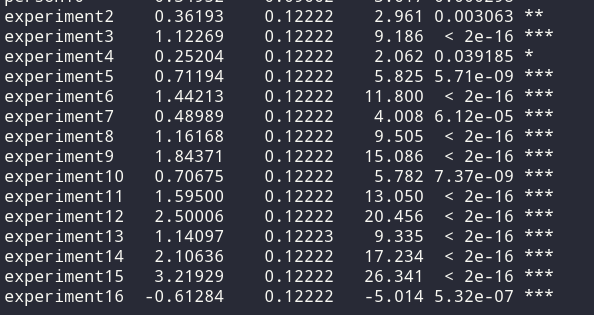
\includegraphics[width=.7\linewidth]{p1_anova_summay}
\end{figure}


Yes, experiment is significant.\\
	
-- All experiments are (at 5\pro) significantly different from the control experiment which has been set to reference

\section{Discussion}
\subsection{Classification of persons}
--Plot: Seems nonlinear (parabolic data)\\
-- Plot: For humans: Easy difference in \(y\)-coordinate between first repetitions of the two initial test subjects.

\subsection{Test of difference in experiments}
-- Expectation: Yes, significant difference as 15 different obtacle avoidance tests + control is considered\\
-- Surprise: Repetition is also significant though\\
-- Which coordinate it is explains the largest part of data variability but experiment no. comes in second\\
-- Low residual variance when compared to within-group variance\\
-- Model assumptions: Plot\\
\begin{thebibliography}{9}
	\bibitem{Tue} Herlau, Tue et al. "Introduction to Machine Learning and Data Mining: Lecture notes, Fall 2019, version 1.4b" 13/12-19.
	\bibitem{KNN} Ripley, Brian: "Package ’class’", 01/01-19 .\\
	At:
	\url{https://cran.r-project.org/web/packages/class/class.pdf} (consulted 16/01-20)
	\bibitem{Tree} Ripley, Brian: "Package ‘tree’", 26/05-19.\\ At: \url{https://cran.r-project.org/web/packages/tree/tree.pdf} (consulted 16/01-20)
	\bibitem{Deviance} Ritschard, Gilbard: "Computing and using the deviance with classification trees", 01-06.\\
	 At:
	\url{http://mephisto.unige.ch/pub/publications/gr/ritschard_compstat06.pdf} (consulted 16/01-20)
\end{thebibliography}
\appendix
\section{Appendix: Figures}
\begin{figure}[H]
	
	\centering
	\subfloat{
		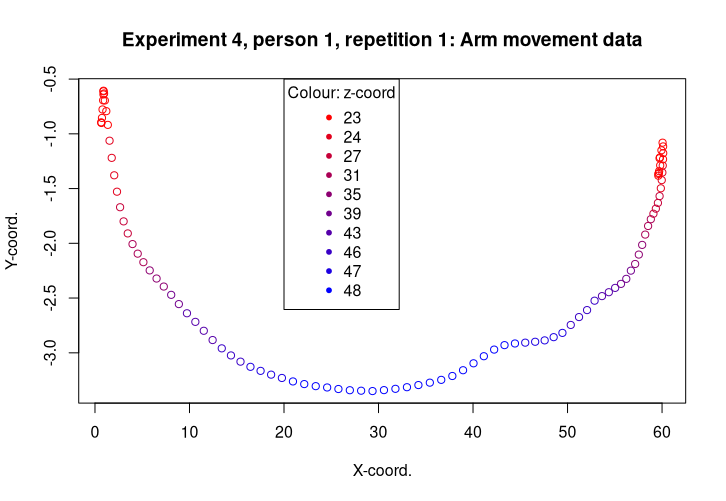
\includegraphics[width=.5\linewidth]{p1_example}
	}
	\subfloat{5
		\centering
		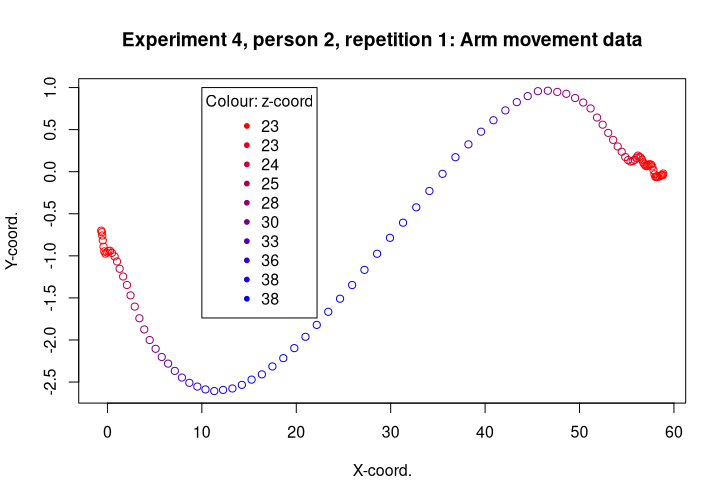
\includegraphics[width=.5\linewidth]{p1_example2}
	}
	\caption{Floats}
	\label{fig:2dtrajects}
\end{figure}


\end{document}

















